% !TeX program = xelatex
\documentclass[10pt]{beamer}

\usetheme{metropolis}

\usepackage{pgfplots}
\usepgfplotslibrary{fillbetween}
\usepackage{pgfopts}
\usepackage{amsmath}
\usepackage{structuralanalysis}
\usepackage{tikz}
\usepackage{tikz-3dplot}
\usepackage{chngcntr}
\usepackage{wasysym}
\usepackage{mathtools}
\usepackage{alphalph}
\usepackage{xcolor}
\usepackage[showdow=false, en-US]{datetime2}

\newcommand{\highlight}[1]{%
	\colorbox{red!50}{$\displaystyle#1$}}

\setcounter{lecture}{7}
\counterwithin{equation}{lecture}
\makeatletter
\def\user@resume{resume}
\def\user@intermezzo{intermezzo}
%
\newcounter{previousequation}
\newcounter{lastsubequation}
\newcounter{savedparentequation}
\setcounter{savedparentequation}{1}
% 
\renewenvironment{subequations}[1][]{%
	\def\user@decides{#1}%
	\setcounter{previousequation}{\value{equation}}%
	\ifx\user@decides\user@resume 
	\setcounter{equation}{\value{savedparentequation}}%
	\else  
	\ifx\user@decides\user@intermezzo
	\refstepcounter{equation}%
	\else
	\setcounter{lastsubequation}{0}%
	\refstepcounter{equation}%
	\fi\fi
	\protected@edef\theHparentequation{%
		\@ifundefined {theHequation}\theequation \theHequation}%
	\protected@edef\theparentequation{\theequation}%
	\setcounter{parentequation}{\value{equation}}%
	\ifx\user@decides\user@resume 
	\setcounter{equation}{\value{lastsubequation}}%
	\else
	\setcounter{equation}{0}%
	\fi
	\def\theequation  {\theparentequation  \alph{equation}}%
	\def\theHequation {\theHparentequation \alph{equation}}%
	\ignorespaces
}{%
%  \arabic{equation};\arabic{savedparentequation};\arabic{lastsubequation}
\ifx\user@decides\user@resume
\setcounter{lastsubequation}{\value{equation}}%
\setcounter{equation}{\value{previousequation}}%
\else
\ifx\user@decides\user@intermezzo
\setcounter{equation}{\value{parentequation}}%
\else
\setcounter{lastsubequation}{\value{equation}}%
\setcounter{savedparentequation}{\value{parentequation}}%
\setcounter{equation}{\value{parentequation}}%
\fi\fi
%  \arabic{equation};\arabic{savedparentequation};\arabic{lastsubequation}
\ignorespacesafterend
}
\makeatother
\title{AE 737 - Mechanics of Damage Tolerance}
\subtitle{Lecture \arabic{lecture}}
\date{Last Updated: \today\ at \DTMcurrenttime}
\author{Dr. Nicholas Smith}
\institute{Wichita State University, Department of Aerospace Engineering}
% \titlegraphic{\hfill\includegraphics[height=1.5cm]{logo/logo}}

\begin{document}

\maketitle

\begin{frame}{homework review}
	\begin{itemize}
		\item Don't cover problem number with staple
		\item Clearly indicate solution
	\end{itemize}
\end{frame}

\begin{frame}{schedule}
	\begin{itemize}
		\item 11 Feb - Fracture Toughness
		\item 16 Feb - Residual Strength, Homework 3 Due, Homework 4 Assigned
		\item 18 Feb - Residual Strength
		\item 23 Feb - Multiple Site Damage, Homework 4 Due, Homework 5 Assigned
		\item 25 Feb - Mixed-mode Fracture
	\end{itemize}
\end{frame}

\begin{frame}
  \frametitle{outline}
  \setbeamertemplate{section in toc}[sections numbered]
  \tableofcontents[hideallsubsections]
\end{frame}

\section{R-curve}

\begin{frame}{R-curve}
	\begin{itemize}[<+->]
		\item For materials with some plasticity, the $K_R$ Curve, or R Curve, is very important
		\item Sometimes called a "resistance curve" it is generally dependent on
		\begin{itemize}[<+->]
			\item Thickness
			\item Temperature
			\item Strain rate
		\end{itemize}
		\item When done correctly, $K_R$ curves are not dependent on initial crack size or the specimen type used
		\item ASTM E561
	\end{itemize}
\end{frame}

\begin{frame}{$K_c$}
	\begin{itemize}[<+->]
		\item While we can look up plane stress $K_c$ for various materials, it is best if we have a $K_R$ curve
		\item We may not know if the table uses $K_c$ using the tangent intersection method, or maximum stress intensity
		\item Even if tangent intersection method is used, $K_c$ will different somewhat based on initial crack length
	\end{itemize}
\end{frame}

\begin{frame}{R-curve}
	\begin{itemize}
		\item There are two main methods for plotting the R-curve
		\item Crack size is measured directly (possibly with a drawn-on scale and camera)
		\item Effective crack size is calculated from the load-displacement data
	\end{itemize}
\end{frame}

\begin{frame}{physical crack}
	\begin{itemize}
		\item When the physical crack size is measured, we need to calculate the effective crack length (and effective stress intensity factor) at each data point
		\item The effective crack length calculated from the load-displacement data already has the plastic zone effect built in
	\end{itemize}
\end{frame}

\begin{frame}{secant compliance M(T)}
	\begin{itemize}[<+->]
		\item Using the slope data from our load-displacement curve, we can calculate the effective crack length using
		\begin{multline}
		EB\left(\frac{\Delta v}{\Delta P}\right) = \frac{2 Y}{W} \sqrt{\frac{\pi a / W}{\sin (\pi a / W)}} \\
		\qquad \left[\frac{2W}{\pi Y} \cosh^{-1} \left(\frac{\cosh(\pi Y/W)}{\cos (\pi a / W)}\right) - \frac{1+\nu}{\sqrt{1 + \left(\frac{\sin(\pi a/W)}{\sinh (\pi Y/W)}\right)^2}}+\nu\right]
		\end{multline}
	\end{itemize}
\end{frame}

\begin{frame}{secant compliance M(T)}
	\begin{itemize}[<+->]
		\item This equation is difficult to solve directly for $a$ (for M(T) specimens) 
		\item Instead it is generally solved iteratively
		\item The following equations are used to give a good initial guess to use in iterations
		\begin{align}
		X &= 1 - \exp \left[\frac{-\sqrt{[EB(\Delta v/ \Delta P)]^2 - (2Y/W)^2}}{2.141}\right]\\
		&\begin{aligned}
		\mathllap{\frac{2a}{W}} &= 1.2235X - 0.699032X^2 + 3.25584X^3 - 6.65042X^4 + \\
		&\qquad5.54X^5 - 1.66989X^6
		\end{aligned}
		\end{align}
	\end{itemize}
\end{frame}

\begin{frame}{secant compliance M(T)}
	\begin{itemize}
		\item In the above equations, the following are the definitions of parameters used
		\begin{align*}
		E &= \qquad \text{Young's Modulus}\\
		\Delta v / \Delta P &= \qquad \text{specimen compliance}\\
		B &= \qquad \text{specimen thickness}\\
		W &= \qquad \text{specimen width}\\
		Y &= \qquad \text{half span of the displacement measurement points}\\
		a &= \qquad \text{effective crack length}\\
		\nu &= \qquad \text{Poisson's ratio}
		\end{align*}
	\end{itemize}
\end{frame}

\begin{frame}{secant compliance C(T)}
	\begin{itemize}[<+->]
		\item For C(T) specimens, we use the following equations
		\item[]
		\begin{equation}
		EB\frac{\Delta v}{\Delta P} = A_0 + A_1\left(\frac{a}{W}\right) + A_2\left(\frac{a}{W}\right)^2 + A_3\left(\frac{a}{W}\right)^3 + A_4\left(\frac{a}{W}\right)^4
		\end{equation}
		\item The coefficients will differ based on where the displacement is measured from
	\end{itemize}
\end{frame}

\begin{frame}{secant compliance C(T)}
	\begin{figure}
		\centering
		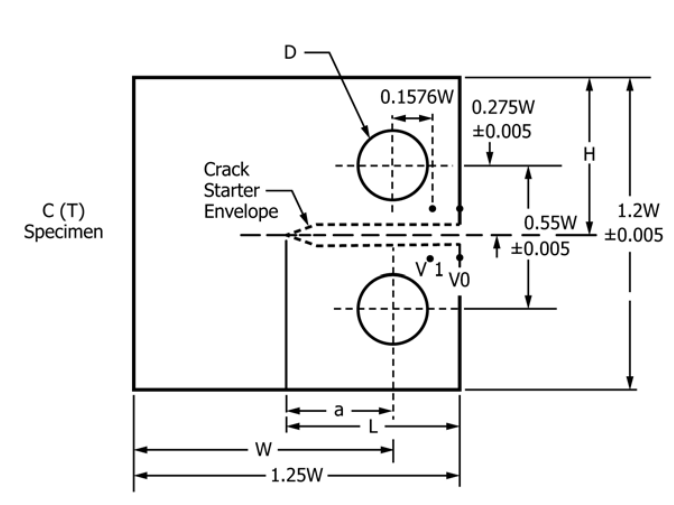
\includegraphics[width=0.7\linewidth]{CT-KR}
		\label{fig:CT-KR}
	\end{figure}
\end{frame}

\begin{frame}{secant compliance C(T)}
	\begin{tabular}{rrrrrr}
		location	& $A_0$ & $A_1$ & $A_2$ & $A_3$ & $A_4$ \\ 
		\hline
		$V_0$	& 120.7 & -1065.3 & 4098.0 & -6688.0 & 4450.5 \\ 
		$V_1$	& 103.8 & -930.4 & 3610.0 & -5930.5 & 3979.0
	\end{tabular} 
	\begin{tabular}{rrrrrrr}
		location	& $C_0$ & $C_1$ & $C_2$ & $C_3$ & $C_4$ & $C_5$ \\ 
		\hline
		$V_0$	& 1.0010 & -4.6695 & 18.460 & -236.82 & 1214.90 & -2143.6\\ 
		$V_1$	& 1.0008 & -4.4473 & 15.400 & -180.55 & 870.92 & -1411.3
	\end{tabular} 
\end{frame}

\begin{frame}{secant compliance C(T)}
	\begin{itemize}
		\item Where the initial guess for $a$ is provided by
		\begin{equation}
		\frac{a}{W} = C_0 + C_1 U + C_2 U^2 + C_3 U^3 + C_4 U^4 + C_5 U^5
		\end{equation}
		\item and $U$ is given by
		\begin{equation}
		U = \frac{1}{1 + \sqrt{EB\frac{\Delta v}{\Delta P}}}
		\end{equation}
	\end{itemize}
\end{frame}

\section{superposition}

\begin{frame}{superposition vs. compounding}
	\begin{itemize}
		\item In this course, we use "superposition" to combine various loading conditions
		\item We use "compounding" to combine various edge effects
		\item Both are very powerful tools and important concepts
	\end{itemize}
\end{frame}

\begin{frame}{superposition}
	\begin{itemize}
		\item Sometimes we have to think out of the box to come up with a superposition
		\item Note: every super-posed solution must still satisfy equilibrium!
		\item On-board example: pressurized crack
	\end{itemize}
\end{frame}

\begin{frame}{group 1}
\begin{figure}
\centering
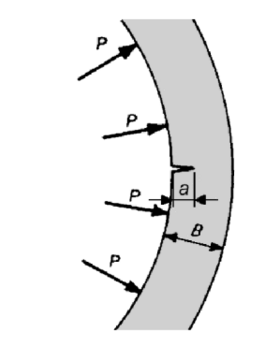
\includegraphics[width=0.3\linewidth]{group1}
\caption{semi-elliptical surface flaw in a pressurized cylinder}
\label{fig:group1}
\end{figure}
\end{frame}

\begin{frame}{group 2}
	\begin{figure}
		\centering
		\begin{tikzpicture}
		\begin{scope}[scale=1.5]
		\draw (0,0) -- (0,1) -- (4,1) -- (4,-1) -- (0,-1) -- (0,0);
		\draw (0,0) -- (0.5,0);
		\draw node at (0.25,0.2) {a};
		\draw[->] (1,0.5) -- (1,1.5) node[above] {$P$};
		\draw[->] (1,-0.5) -- (1,-1.5) node[below] {$P$};
		\end{scope}
		\end{tikzpicture}
		\caption{off-center point load on an edge-crack (like in a compact tension specimen)}
	\end{figure}
\end{frame}

\begin{frame}{group 3}
	\begin{figure}
		\centering
		\begin{tikzpicture}
		\begin{scope}[scale=2]
		\point{a}{0}{-3.25};
		\point{b}{2}{-3.25};
		\draw (0,-1) -- (0,1) -- (1,1) -- (1,-1) -- (0,-1);
		\draw (0.3,0) -- (0.7,0);
		\draw[->] (0.5,0.2) -- (0.5,0.6) node[above] {P};
		\draw node at (0.5,-0.1) {$2a$};
		\lineload{3}{a}{b}[.25][.25];
		\draw node at (0.5,-1.5) {$\sigma$};
		\end{scope}
		\end{tikzpicture}
	\caption{crack with applied force on one side and a remote stress on the other}
	\end{figure}
\end{frame}

\begin{frame}{group 4}
	\begin{figure}
		\begin{tikzpicture}
		\begin{scope}[scale=.75]
		\draw (0,-1.5) -- (0,1.5) -- (6,1.5) -- (6,-1.5) -- (0,-1.5);
		\draw[->] (3,1.5) -- (3,2) node[above] {$\sigma_1$};
		\draw[->] (3,-1.5) -- (3,-2) node[below] {$\sigma_2$};
		\draw (3,0) circle (0.5);
		\draw (3.5,0) -- (4,0);
		\draw (2.5,0) -- (2,0);
		\draw node at (3,0.7) {D};
		\draw[->] (3,-0.7) node[below]{$P$} -- (3,0);
		\draw[->] (3.2,0.7) -- (3.5,0.7);
		\draw[->] (2.8,0.7) -- (2.5,0.7);
		\end{scope}
		\end{tikzpicture}
		\caption{pin-loaded hole, find superposition such that remote stresses and local forces are separated}
	\end{figure}
\end{frame}
%pin loaded hole (in terms of only \sigma and P)

\section{compounding}

\begin{frame}{compounding}
	\begin{itemize}
		\item Different types of boundaries create different correction factors to the usual stress intensity factor
		\item We often use $\beta$ to indicate the total correction factor
		\item When multiple boundaries are present, we can combine them into one effective correction factor
		\item There are two general methods we use to create a compound correction factor
	\end{itemize}
\end{frame}

\begin{frame}{compounding method 1}
	\begin{itemize}
		\item The first method uses linear superposition, and thus is restricted to cases where the effect of each boundary can be assumed to add linearly
		\item While in most cases this is not strictly true, it provides a reasonable approximation
		\begin{equation}
		K_r = \bar{K} + \sum_{i=1}^{N}(K_i - \bar{K})
		\end{equation}
		\item Where $N$ is the number of boundaries, $\bar{K}$ is the stress intensity factor with no boundaries present and $K_i$ is the stress intensity factor associated with the $i^{\text{th}}$ boundary.
	\end{itemize}
\end{frame}

\begin{frame}{compounding method 1}
	\begin{itemize}
		\item We can rewrite this equation as
		\begin{equation}
		K_r = \sigma \sqrt{\pi a} \beta_r = \sigma \sqrt{\pi a} + \sum_{i=1}^{N}(\sigma \sqrt{\pi a}\beta_i - \sigma \sqrt{\pi a})
		\end{equation}
		\item Which leads to an expression for $\beta_r$ as
		\begin{equation}
		\beta_r = 1+\sum_{i=1}^{N} (\beta_i - 1)
		\end{equation}
	\end{itemize}
\end{frame}

\begin{frame}{compounding method 2}
	\begin{itemize}
		\item An alternative empirical method approximates the boundary effect as
		\begin{equation}
		\beta_r = \beta_1 \beta_2 ... \beta_N
		\end{equation}
		\item If there is no interaction between the boundaries, method 1 and method 2 will give the same result
	\end{itemize}
\end{frame}
%Hand-draw examples from book

\begin{frame}{group 1}
		\begin{figure}[H]
			\centering
			\begin{tikzpicture}
			\begin{scope}[scale=1.5]
			\point{a}{0}{2};
			\point{b}{3}{2};
			\point{c}{0}{-3};
			\point{d}{3}{-3};
			\draw (0,0) -- (0,1) -- (2,1) -- (2,-1) -- (0,-1) -- (0,0);
			\draw (0.2,0) -- (0.8,0);
			\draw node at (0.15,0.1) {\small A} node at (.85,.1) {\small B} node at (.25,.5) {\small $b$};
			\draw node at (0.5,-0.2) {2a};
			\lineload{3}{a}{b}[-.5][-.5];
			\draw node at (1,2) {$\sigma$};
			\lineload{3}{c}{d}[.5][.5];
			\draw node at (1,-2) {$\sigma$};
			\draw[->] (0.7,-0.7) -- (0,-0.7);
			\draw[->] (1.3,-0.7) -- (2,-0.7);
			\draw node at (1,-0.7) {$W$};
			\draw[dashed] (.5,0) -- (.5,.8);
			\draw[->] (0.15,.5) -- (0,.5);
			\draw[->] (.35,.5) -- (.5,.5);
			\draw node at (2.2,0) {$h$};
			\draw[->] (2.2,0.5) -- (2.2,1);
			\draw[->] (2.2,-0.5) -- (2.2,-1);
			\end{scope}
			\end{tikzpicture}
			\caption{off-center crack, finite height}
		\end{figure}
\end{frame}
%off-center crack, finite height

\begin{frame}{group 2}
	\begin{figure}[H]
		\centering
		\begin{tikzpicture}
		\begin{scope}[scale=1.5]
		\point{a}{0}{2};
		\point{b}{3}{2};
		\point{c}{0}{-3};
		\point{d}{3}{-3};
		\draw (0,0) -- (0,1) -- (2,1) -- (2,-1) -- (0,-1) -- (0,0);
		\draw (0.2,0) -- (0.8,0);
		\draw node at (0.15,0.1) {\small A} node at (.85,.1) {\small B} node at (.25,.5) {\small $b$};
		\draw node at (0.5,-0.2) {2a};
		\lineload{3}{a}{b}[-.5][-.5];
		\draw node at (1,2) {$\sigma$};
		\lineload{3}{c}{d}[.5][.5];
		\draw node at (1,-2) {$\sigma$};
		\draw[->] (0.7,-0.7) -- (0,-0.7);
		\draw[->] (1.3,-0.7) -- (2,-0.7);
		\draw node at (1,-0.7) {$W$};
		\draw[dashed] (.5,0) -- (.5,.8);
		\draw[->] (0.15,.5) -- (0,.5);
		\draw[->] (.35,.5) -- (.5,.5);
		\draw (1.5,0) circle (0.25);
		\end{scope}
		\end{tikzpicture}
		\caption{off-center crack, near a hole}
	\end{figure}
\end{frame}
%off-center crack, near hole

\begin{frame}{group 3}
	\begin{figure}[H]
		\centering
		\begin{tikzpicture}
		\begin{scope}[scale=1.5]
		\point{a}{0}{2};
		\point{b}{6}{2};
		\point{c}{0}{-3};
		\point{d}{6}{-3};
		\draw (0,0) -- (0,1) -- (4,1) -- (4,-1) -- (0,-1) -- (0,0);
		\draw (1.5,0) -- (2.5,0);
		\draw node at (2,0.2) {2a};
		\lineload{3}{a}{b}[-.5][-.5];
		\draw node at (2,2) {$\sigma$};
		\lineload{3}{c}{d}[.5][.5];
		\draw node at (2,-2) {$\sigma$};
		\draw (3,0) circle (0.25);
		\draw node at (1,0) {$h$};
		\draw[->] (1,0.5) -- (1,1);
		\draw[->] (1,-0.5) -- (1,-1);
		\end{scope}
		\end{tikzpicture}
		\caption{centered crack, near a hole, finite height}
	\end{figure}
\end{frame}
%centered crack, near hole, finite height

\begin{frame}{group 4}
	\begin{figure}[H]
		\centering
		\begin{tikzpicture}
		\begin{scope}[scale=1.5]
		\point{a}{0}{2};
		\point{b}{6}{2};
		\point{c}{0}{-3};
		\point{d}{6}{-3};
		\draw (0,0) -- (0,1) -- (4,1) -- (4,-1) -- (0,-1) -- (0,0);
		\draw (1.5,0) -- (2.5,0);
		\draw node at (2,0.2) {2a};
		\lineload{3}{a}{b}[-.5][-.5];
		\draw node at (2,2) {$\sigma$};
		\lineload{3}{c}{d}[.5][.5];
		\draw node at (2,-2) {$\sigma$};
		\draw (3,0) circle (0.25);
		\draw (1,0) circle (0.35);
		\end{scope}
		\end{tikzpicture}
		\caption{centered crack, near two holes}
	\end{figure}
\end{frame}
%centered crack, near two holes

\end{document}
